\documentclass[10pt,oneside]{article}
\usepackage[T1]{fontenc}
\usepackage[utf8]{inputenc}
% \usepackage{lmodern}
%\usepackage[adobe-utopia,uppercase=upright,greeklowercase=upright]{mathdesign}
\usepackage[adobe-utopia]{mathdesign}
%\usepackage{minionpro}
% \usepackage{pifont}
% \usepackage{amssymb}
\usepackage{amsmath}
\usepackage[francais]{babel}
% \usepackage[francais]{varioref}
\usepackage[dvips]{graphicx}

\usepackage{framed}
\usepackage[normalem]{ulem}
\usepackage{fancyhdr}
\usepackage{titlesec}
\usepackage{vmargin}
\usepackage{longtable}

\usepackage{ifthen}


%\usepackage{epsfig}
\usepackage{subfig}

\usepackage{multirow}
\usepackage{multicol} % Portions de texte en colonnes
\usepackage{flafter}%floatants après la référence



\usepackage{color}
\usepackage{colortbl}


\definecolor{gris25}{gray}{0.75}
\definecolor{bleu}{RGB}{18,33,98}
\definecolor{bleuf}{RGB}{42,94,171}
\definecolor{bleuc}{RGB}{231,239,247}
\definecolor{rougef}{RGB}{185,18,27}
\definecolor{rougec}{RGB}{255,230,231}
\definecolor{vertf}{RGB}{103,126,82}
\definecolor{vertc}{RGB}{220,255,191}

\newenvironment{rem}[1][\hsize]%
{%
    \def\FrameCommand
    {%
\rotatebox{90}{\textit{\textsf{Remarque}}} 
        {\color{bleuf}\vrule width 3pt}%
        \hspace{0pt}%must no space.
        \fboxsep=\FrameSep\colorbox{bleuc}%
    }%
    \MakeFramed{\hsize#1\advance\hsize-\width\FrameRestore}%
}%
{\endMakeFramed}%


\newenvironment{savoir}[1][\hsize]%
{%
    \def\FrameCommand
    {%
\rotatebox{90}{\textit{\textsf{Savoir}}} 
        {\color{bleuf}\vrule width 3pt}%
        \hspace{0pt}%must no space.
        \fboxsep=\FrameSep\colorbox{bleuc}%
    }%
    \MakeFramed{\hsize#1\advance\hsize-\width\FrameRestore}%
}%
{\endMakeFramed}%

\newenvironment{prob}[1][\hsize]%
{%
    \def\FrameCommand%
    {%
\rotatebox{90}{\textit{\textsf{ Problématique}}} 
        {\color{rougef}\vrule width 3pt}%
        \hspace{0pt}%must no space.
        \fboxsep=\FrameSep\colorbox{rougec}%
    }%
    \MakeFramed{\hsize#1\advance\hsize-\width\FrameRestore}%
}%
{\endMakeFramed}%

\newenvironment{obj}[1][\hsize]%
{%
    \def\FrameCommand%
    {%
\rotatebox{90}{\textit{\textsf{ $\;$}}} 
        {\color{rougef}\vrule width 3pt}%
        \hspace{0pt}%must no space.
        \fboxsep=\FrameSep\colorbox{rougec}%
    }%
    \MakeFramed{\hsize#1\advance\hsize-\width\FrameRestore}%
}%
{\endMakeFramed}%

\newenvironment{defi}[1][\hsize]%
{%
    \def\FrameCommand%
    {%
\rotatebox{90}{\textit{\textsf{Définition\\}}} 
        {\color{bleuf}\vrule width 3pt}%
        \hspace{0pt}%must no space.
        \fboxsep=\FrameSep\colorbox{bleuc}%
    }%
    \MakeFramed{\hsize#1\advance\hsize-\width\FrameRestore}%
}%
{\endMakeFramed}%


\newenvironment{hypo}[1][\hsize]%
{%
    \def\FrameCommand%
    {%
\rotatebox{90}{\textit{\textsf{Hypothèse\\}}} 
        {\color{bleuf}\vrule width 3pt}%
        \hspace{0pt}%must no space.
        \fboxsep=\FrameSep\colorbox{bleuc}%
    }%
    \MakeFramed{\hsize#1\advance\hsize-\width\FrameRestore}%
}%
{\endMakeFramed}%


\newenvironment{prop}[1][\hsize]%
{%
    \def\FrameCommand%
    {%
\rotatebox{90}{\textit{\textsf{Propriété\\}}} 
        {\color{bleuf}\vrule width 3pt}%
        \hspace{0pt}%must no space.
        \fboxsep=\FrameSep\colorbox{bleuc}%
    }%
    \MakeFramed{\hsize#1\advance\hsize-\width\FrameRestore}%
}%
{\endMakeFramed}%

\newenvironment{props}[1][\hsize]%
{%
    \def\FrameCommand%
    {%
\rotatebox{90}{\textit{\textsf{Propriétés\\}}} 
        {\color{bleuf}\vrule width 3pt}%
        \hspace{0pt}%must no space.
        \fboxsep=\FrameSep\colorbox{bleuc}%
    }%
    \MakeFramed{\hsize#1\advance\hsize-\width\FrameRestore}%
}%
{\endMakeFramed}%

\newenvironment{exemple}[1][\hsize]%
{%
    \def\FrameCommand%
    {%
\rotatebox{90}{\textit{\textsf{Exemple\\}}} 
        {\color{vertf}\vrule width 3pt}%
        \hspace{0pt}%must no space.
        \fboxsep=\FrameSep\colorbox{vertc}%
    }%
    \MakeFramed{\hsize#1\advance\hsize-\width\FrameRestore}%
}%
{\endMakeFramed}%

\newenvironment{resultat}[1][\hsize]%
{%
    \def\FrameCommand%
    {%
\rotatebox{90}{\textit{\textsf{Résultat\\}}} 
        {\color{rougef}\vrule width 3pt}%
        \hspace{0pt}%must no space.
        \fboxsep=\FrameSep\colorbox{rougec}%
    }%
    \MakeFramed{\hsize#1\advance\hsize-\width\FrameRestore}%
}%
{\endMakeFramed}%

\newenvironment{methode}[1][\hsize]%
{%
    \def\FrameCommand%
    {%
\rotatebox{90}{\textit{\textsf{Méthode\\}}} 
        {\color{rougef}\vrule width 3pt}%
        \hspace{0pt}%must no space.
        \fboxsep=\FrameSep\colorbox{rougec}%
    }%
    \MakeFramed{\hsize#1\advance\hsize-\width\FrameRestore}%
}%
{\endMakeFramed}%

\newenvironment{theo}[1][\hsize]%
{%
    \def\FrameCommand%
    {%
\rotatebox{90}{\textit{\textsf{Théorème\\}}} 
        {\color{rougef}\vrule width 3pt}%
        \hspace{0pt}%must no space.
        \fboxsep=\FrameSep\colorbox{rougec}%
    }%
    \MakeFramed{\hsize#1\advance\hsize-\width\FrameRestore}%
}%
{\endMakeFramed}%

\newenvironment{warn}[1][\hsize]%
{%
    \def\FrameCommand%
    {%
\rotatebox{90}{\textit{\textsf{Attention\\}}} 
        {\color{rougef}\vrule width 3pt}%
        \hspace{0pt}%must no space.
        \fboxsep=\FrameSep\colorbox{rougec}%
    }%
    \MakeFramed{\hsize#1\advance\hsize-\width\FrameRestore}%
}%
{\endMakeFramed}%

% \usepackage{pstricks}
%\usepackage{minitoc}
% \setcounter{minitocdepth}{4}

\setcounter{tocdepth}{2}

% \mtcselectlanguage{french} 

%\usepackage{draftcopy}% "Brouillon"
% \usepackage{floatflt}
\usepackage{psfrag}
%\usepackage{listings} % Permet d'insérer du code de programmation
\renewcommand{\baselinestretch}{1.2}

% Changer la numérotation des figures :
% ------------------------------------
% \makeatletter
% \renewcommand{\thefigure}{\ifnum \c@section>\z@ \thesection.\fi
%  \@arabic\c@figure}
% \@addtoreset{figure}{section}
% \makeatother
 


%%%%%%%%%%%%
% Définition des vecteurs %
%%%%%%%%%%%%
 \newcommand{\vect}[1]{\overrightarrow{#1}}

%%%%%%%%%%%%
% Définition des torseusr %
%%%%%%%%%%%%

 \newcommand{\torseur}[1]{%
\left\{{#1}\right\}
}

\newcommand{\torseurcin}[3]{%
\left\{\mathcal{#1} \left(#2/#3 \right) \right\}
}

\newcommand{\torseurstat}[3]{%
\left\{\mathcal{#1} \left(#2\rightarrow #3 \right) \right\}
}

 \newcommand{\torseurc}[8]{%
%\left\{#1 \right\}=
\left\{
{#1}
\right\}
 = 
\left\{%
\begin{array}{cc}%
{#2} & {#5}\\%
{#3} & {#6}\\%
{#4} & {#7}\\%
\end{array}%
\right\}_{#8}%
}

 \newcommand{\torseurcol}[7]{
\left\{%
\begin{array}{cc}%
{#1} & {#4}\\%
{#2} & {#5}\\%
{#3} & {#6}\\%
\end{array}%
\right\}_{#7}%
}

 \newcommand{\torseurl}[3]{%
%\left\{\mathcal{#1}\right\}_{#2}=%
\left\{%
\begin{array}{l}%
{#1} \\%
{#2} %
\end{array}%
\right\}_{#3}%
}

 \newcommand{\vectv}[3]{%
\vect{V\left( {#1} \in {#2}/{#3}\right)}
}


\newcommand{\vectf}[2]{%
\vect{R\left( {#1} \rightarrow {#2}\right)}
}

\newcommand{\vectm}[3]{%
\vect{\mathcal{M}\left( {#1}, {#2} \rightarrow {#3}\right)}
}


 \newcommand{\vectg}[3]{%
\vect{\Gamma \left( {#1} \in {#2}/{#3}\right)}
}

 \newcommand{\vecto}[2]{%
\vect{\Omega\left( {#1}/{#2}\right)}
}
% }$$\left\{\mathcal{#1} \right\}_{#2} =%
% \left\{%
% \begin{array}{c}%
%  #3 \\%
%  #4 %
% \end{array}%
% \right\}_{#5}}

%  ------------------------------------------
% | Modification du formatage des sections : | 
%  ------------------------------------------

% Grands titres :
% ---------------

\newcommand{\titre}[1]{%
\begin{center}
      \bigskip
      \rule{\textwidth}{1pt}
      \par\vspace{0.1cm}
      
      \textbf{\large #1}
      \par\rule{\textwidth}{1pt}
    \end{center}
    \bigskip
  }

% Supprime le numéro du chapitre dans la numérotation des sections:
% -----------------------------------------------------------------
\makeatletter
\renewcommand{\thesection}{\@arabic\c@section}
\makeatother


% \titleformat{\chapter}[display]
% {\normalfont\Large\filcenter}
% {}
% {1pc}
% {\titlerule[1pt]
%   \vspace{1pc}%
%   \Huge}[\vspace{1ex}%
% \titlerule]


%%%% Chapitres Comme PY Pechard %%%%%%%%%
% numéro du chapitre
\DeclareFixedFont{\chapnumfont}{OT1}{phv}{b}{n}{80pt}
% pour le mot « Chapitre »
\DeclareFixedFont{\chapchapfont}{OT1}{phv}{m}{it}{40pt}
% pour le titre
\DeclareFixedFont{\chaptitfont}{T1}{phv}{b}{n}{25pt}

\definecolor{gris}{gray}{0.75}
\titleformat{\chapter}[display]%
	{\sffamily}%
	{\filleft\chapchapfont\color{gris}\chaptertitlename\
	\\
	\vspace{12pt}
	\chapnumfont\thechapter}%
	{16pt}%
	{\filleft\chaptitfont}%
	[\vspace{6pt}\titlerule\titlerule\titlerule]

%%%%  Fin Chapitres Comme PY Pechard %%%%%%%%%


% Section, subsection, subsubsection sans serifs :
% % ----------------------------------------------

% \makeatletter
% \renewcommand{\section}{\@startsection{section}{0}{0mm}%
% {\baselineskip}{.3\baselineskip}%
% {\normalfont\sffamily\Large\textbf}}%
% \makeatother

\makeatletter
\renewcommand{\@seccntformat}[1]{{\textcolor{bleu}{\csname
the#1\endcsname}\hspace{0.5em}}}
\makeatother

\makeatletter
\renewcommand{\section}{\@startsection{section}{1}{\z@}%
                       {-4ex \@plus -1ex \@minus -.4ex}%
                       {1ex \@plus.2ex }%
                       {\normalfont\Large\sffamily\bfseries}}%
\makeatother
 
\makeatletter
\renewcommand{\subsection}{\@startsection {subsection}{2}{\z@}
                          {-3ex \@plus -0.1ex \@minus -.4ex}%
                          {0.5ex \@plus.2ex }%
                          {\normalfont\large\sffamily\bfseries}}
\makeatother
 
\makeatletter
\renewcommand{\subsubsection}{\@startsection {subsubsection}{3}{\z@}
                          {-2ex \@plus -0.1ex \@minus -.2ex}%
                          {0.2ex \@plus.2ex }%
                          {\normalfont\large\sffamily\bfseries}}
\makeatother
 
\makeatletter             
\renewcommand{\paragraph}{\@startsection{paragraph}{4}{\z@}%
                                    {-2ex \@plus-.2ex \@minus .2ex}%
                                    {0.1ex}%               
{\normalfont\sffamily\bfseries}}
\makeatother
 
\makeatletter
\renewcommand{\subparagraph}{\@startsection{subparagraph}{5}{\z@}%
                                       {-2ex \@plus-.1ex \@minus .2ex}%
                                       {0.1ex}%
				    {\normalfont\normalsize\sffamily\bfseries}}
\makeatletter
% \makeatletter
% \renewcommand{\subsection}{\@startsection{subsection}{1}{2mm}%
% {\baselineskip}{.3\baselineskip}%
% {\normalfont\sffamily\large\textbf}}%
% \makeatother
% 
% \makeatletter
% \renewcommand{\subsubsection}{\@startsection{subsubsection}{2}{4mm}%
% {\baselineskip}{.15\baselineskip}%
% {\normalfont\sffamily\large\textbf}}%
% \makeatother
% 
% \makeatletter
% \renewcommand{\paragraph}{\@startsection{paragraph}{3}{6mm}%
% {\baselineskip}{.15\baselineskip}%
% {\normalfont\sffamily\large\textbf}}%
% \makeatother
 
\setcounter{secnumdepth}{4}


%  --------
% | Marges |
%  --------


% \setmarginsrb{2.5cm}{1.5cm}{2.5cm}{2cm}{1cm}{1cm}{1cm}{1cm}
\setmarginsrb{1.5cm}{1cm}{1cm}{1.5cm}{1cm}{1cm}{1cm}{1cm}

% Changer les marges localement :
% -----------------------------
\newenvironment{changemargin}[2]{\begin{list}{}{%
\setlength{\topsep}{0pt}%
\setlength{\leftmargin}{0pt}%
\setlength{\rightmargin}{0pt}%
\setlength{\listparindent}{\parindent}%
\setlength{\itemindent}{\parindent}%
\setlength{\parsep}{0pt plus 1pt}%
\addtolength{\leftmargin}{#1}%
\addtolength{\rightmargin}{#2}%
}\item }{\end{list}}



\usepackage{pst-solides3d}
\usepackage{titletoc}
\titlecontents{chapter}[+3pc]
  {\addvspace{10pt}\sffamily\bfseries}
{\contentslabel[{\pscirclebox[fillstyle=solid,fillcolor=gray!25,
linecolor=gray!25,framesep=4pt]{\textcolor{white}{\thecontentslabel}}}]{2.5pc}}
  {}
  {\dotfill \normalfont\thecontentspage\ }

\titlecontents{section}[3pc]
  {\addvspace{2pt}\sffamily}
  {\contentslabel[\thecontentslabel]{1.8pc}}
  {}
  {\dotfill \normalfont\thecontentspage\ }

\titlecontents{subsection}[5pc]
  {\addvspace{2pt}\sffamily}
  {\contentslabel[\thecontentslabel]{1.8pc}}
  {}
  {\dotfill \normalfont\thecontentspage\ }

\titlecontents{subsubsection}[8pc]
  {\addvspace{2pt}\sffamily}
  {\contentslabel[\thecontentslabel]{3pc}}
  {}
  {\dotfill \normalfont\thecontentspage\ }
%{\;\titlerule\;\normalfont\thecontentspage\ }

\titlecontents{paragraph}[9pc]
  {\addvspace{2pt}\sffamily}
  {\contentslabel[\thecontentslabel]{3.5pc}}
  {}
  {\dotfill \normalfont\thecontentspage\ }




\usepackage[%
    pdftitle={Statique - DS11},
    pdfauthor={Xavier Pessoles},
    colorlinks=true,
    linkcolor=blue,
    citecolor=magenta]{hyperref}



% \makeatletter \let\ps@plain\ps@empty \makeatother
%% DEBUT DU DOCUMENT
%% =================
\sloppy
\hyphenpenalty 10000

\newcommand{\Pointilles}[1][3]{%
\multido{}{#1}{\makebox[\linewidth]{\dotfill}\\[\parskip]
}}

\begin{document}


\newboolean{prof}
\setboolean{prof}{false}
%------------- En tetes et Pieds de Pages ------------
\pagestyle{fancy}
\renewcommand{\headrulewidth}{0.2pt}

\fancyhead{}
\fancyhead[L]{PTSI -- Sciences Industrielles pour l'Ingénieur}
\fancyhead[R]{Lycée Jules Haag -- Besançon}


\renewcommand{\footrulewidth}{0.2pt}
\fancyfoot[C]{\bfseries \thepage}
\fancyfoot[L]{2010 -- 2011}
\ifthenelse{\boolean{prof}}{%
\fancyfoot[R]{DS 11 -- Statique}
}{%
\fancyfoot[R]{DS 11 -- Statique}
}

%\fancyfoot[RO]{Version du \today}
% \fancyfoot[LE]{Version du \today}
% \fancyfoot[RO]{\textcolor{gris25}{Version rapporteurs}}
% \fancyfoot[LE]{\textcolor{gris25}{Version rapporteurs}}
% \fancyfoot[R]{\textcolor{gris25}{Version rapporteurs}}
% ----------------------------------------------------



\vspace{1cm}

\begin{center}
 \huge\textsc{Devoir Surveillé 11}

\vspace{1cm}

 \large\textsc{Mercredi 15 juin 2011 -- 2 heures}
\end{center}

\vspace{1cm}


\noindent\rule{\linewidth}{.2pt}
\begin{center}
 \large\textbf{CI : 3} \textit{Statique : Modélisation, prévision et vérification du comportement statique des systèmes}

\end{center}
\noindent\rule{\linewidth}{.2pt}


\vfill

\textbf{Contenu du sujet :}
\begin{itemize}
\item \textbf{Statique -- 2 heures}
%\begin{itemize}
%\item Station de  stockage automatique -- 1h30
%\end{itemize}
%\item \textbf{Partie 2 : Conception -- 30 min}
\end{itemize}

\vfill

\textbf{Consignes et recommandations :}
\begin{itemize}
\item \textbf{Il est recommandé de lire le sujet dans son intégralité avant de
répondre aux questions}
\item \textbf{Les question sont numérotées et ordonnées mais beaucoup d'entre elles sont indépendantes.}
%\item \textbf{Il est recommandé de passer une heure sur chacune des parties.}
%\item \textbf{Les parties seront notées proportionnellement aux temps proposés ci-dessus.}
\item \textbf{Il est demandé de :}
\begin{itemize}
\item \textit{rappeler, sur sa copie le numéro de la question avant de développer sa réponse;}
\item \textit{bien respecter l'ensemble des notations alphabétiques et numériques définies dans le sujet et de préciser ses propres notations lorsque cela s'avère nécessaire;}
\item \textit{justifier ses hypothèses, et de rédiger clairement ses réponses.}
%\item de rendre les documents réponse.

\end{itemize}
\end{itemize}

\vfill

\begin{center}
\textsc{\textbf{Tout Document Interdit}}

 \textsc{\textbf{Calculatrices, Téléphones Portables, Lecteur MP3 ...
Interdits.}}

\end{center}

\newpage


\section{Système de positionnement de radar}


\begin{minipage}[c]{.45\linewidth}
Afin d'assurer la sécurité des personnes chargées de déminer les terrains militaires, les ingénieurs ont imaginé d'intégrer un détecteur de métaux à un véhicule blindé. Grâce à ce système, les démineurs peuvent rester à l'abri dans le véhicule ou cas où la mine venait à exploser.
\end{minipage}\hfill
\begin{minipage}[c]{.5\linewidth}
\begin{center}
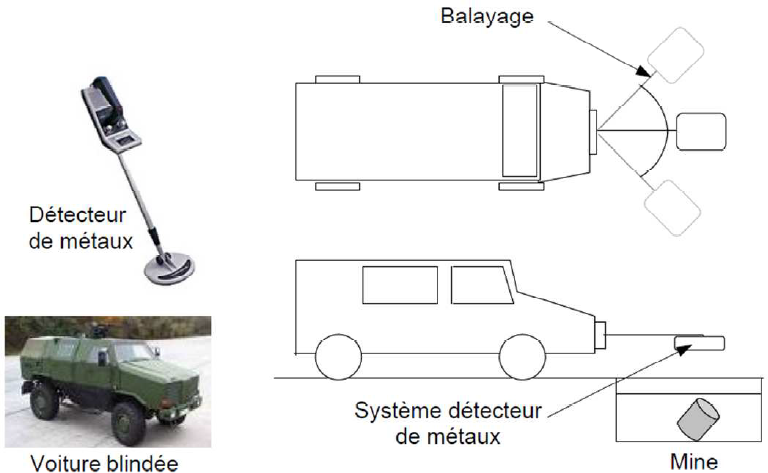
\includegraphics[width=\textwidth]{png/img1}
\end{center}
\end{minipage}

\vspace{.5cm}

On donne ci-dessous le schéma d'architecture de la solution retenue ainsi qu'un extrait du cahier des charges fonctionnel.

\begin{center}
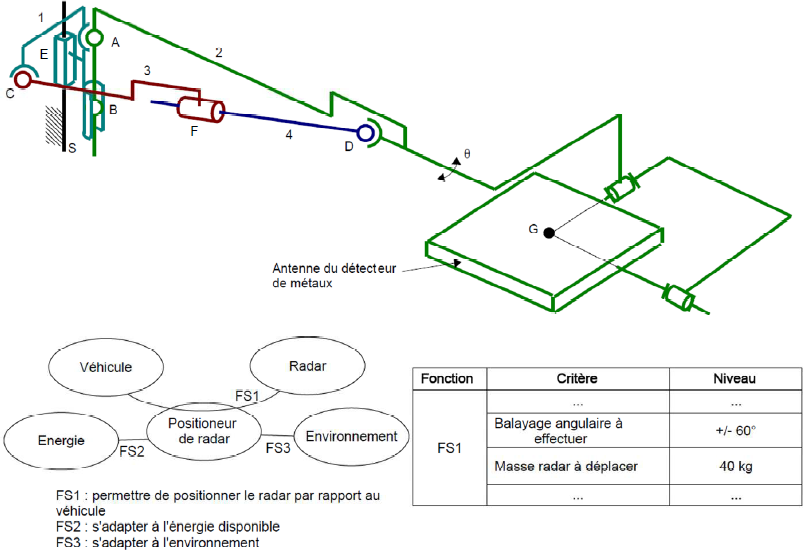
\includegraphics[width=.9\textwidth]{png/img2}
\end{center}

Le balayage par l'antenne de la zone à nettoyer est réalisé grâce à la rotation d'axe $(AB)$ de la pièce 2 actionnée par un vérin hydraulique 3--4. L'antenne du détecteur de métaux est fixée sur un support permettant une double rotation suivant deux axes perpendiculaires de façon à ce qu'elle puisse toujours rester parallèle au sol. Ces deux rotations sont générées par deux moteurs électriques. Le support $S$ est fixé sur le châssis du véhicule par un vérin.

L'objectif de cette étude est de vérifier que le positionneur de radar permet de satisfaire ou non les critères de balayage angulaire à effectuer et de masse de radar à déplacer FS1. 

Hypothèses de modélisation : 
\begin{itemize}
\item la pesanteur n'agit que sur l'antenne de son centre $G$; 
\item la base $(\vect{x_0}, \vect{y_0}, \vect{z_0})$ est liée au sol. Le sol est en pente selon un angle $\alpha=15^o$ par rapport à la verticale ascendante de la base $(\vect{x_g}= \vect{x_0}, \vect{y_g},\vect{z_g})$;
\item la base $(\vect{x_1}, \vect{y_1}, \vect{z_1}=\vect{z_0})$ est liée au véhicule 1 qui se déplace sur le sol selon un angle $\beta$ ($0\leq \beta \leq 2\pi$);
\item la base $(\vect{x_2}, \vect{y_2}, \vect{z_2}=\vect{z_1})$  est liée au bras 2 du positionneur de radar. La position du bras 2 par rapport à la voiture est paramétrée par l'angle $\theta$;
\item la section du vérin 3--4 est notée $S$; 
\item la pression dans le vérin est notée $p$ et est supposée constante;
\item toutes les liaisons sont supposées parfaites.
\end{itemize}


\begin{center}
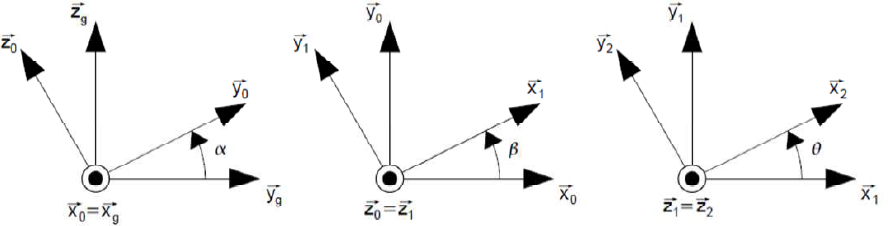
\includegraphics[width=.9\textwidth]{png/img3}
\end{center}

%\subsection*{Etude du critère de masse à déplacer}

\subsection*{Etude du critère de masse à déplacer}

On retient le modèle 3D suivant. Le solide 2 comprend l'antenne et son support orientable. 


\begin{center}
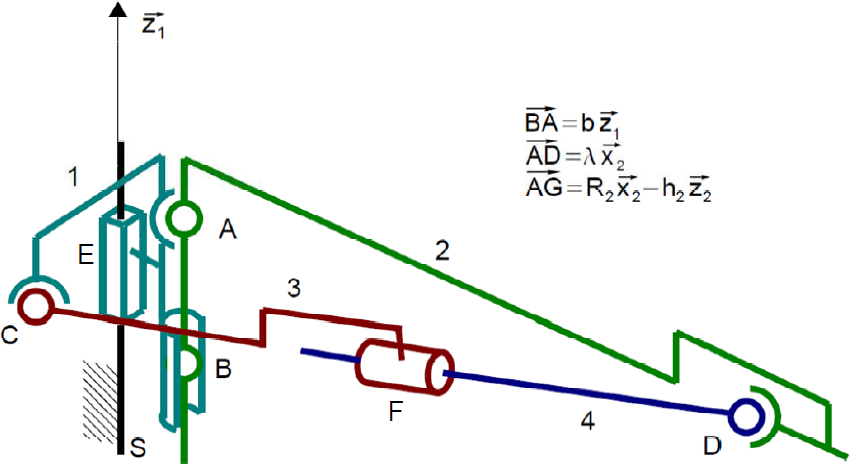
\includegraphics[width=.9\textwidth]{png/img4}
\end{center}

\paragraph{}
\textit{Etablir le graphe de structure du système. Indiquer sur ce graphe le nombre d'inconnues des torseurs d'actions mécaniques transmissibles par chacune des liaisons.}

L'action mécanique transmissible par la liaison rotule $A$ est modélisée par le torseur suivant :
$$
\left\{
F_{\text{rotule 1}\rightarrow 2} 
\right\}=
\left\{
\begin{array}{cc}
X_{12} & 0 \\
Y_{12} & 0 \\
Z_{12} & 0 \\
\end{array}
\right\}_{A,B_1}
$$

L'action mécanique transmissible par la liaison linéaire annulaire en $B$ d'axe $(B,\vect{z_1})$ est modélisée par le torseur suivant :
$$
\left\{
F_{\text{lin annulaire }1\rightarrow 2} 
\right\}=
\left\{
\begin{array}{cc}
X'_{12} & 0 \\
Y'_{12} & 0 \\
0 & 0 \\
\end{array}
\right\}_{B,B_1}
$$

L'action mécanique de la pesanteur sur le solide 2 est modélisée par le torseur suivant :
$$
\left\{
F_{\text{pesanteur }\rightarrow 2} 
\right\}=
\left\{
\begin{array}{cc}
- P \vect{z_g} \\
\vect{0} \\
\end{array}
\right\}_{G}
$$

\paragraph{}
\textit{Donner la forme des torseurs d'actions transmissibles des liaisons 1--3, 3--4 et 2--4 dans la base 3 conformément à la notation imposée ci-dessous.}

Action mécanique exercée par le solide $i$ sir le solide $j$ au point $P$ dans la base 3 :
$$
\left\{
F_{j \rightarrow i} 
\right\}=
\left\{
\begin{array}{cc}
X_{ij} & L_{ij} \\
Y_{ij} & M_{ij} \\
Z_{ij} & N_{ij} \\
\end{array}
\right\}_{P,B_3}
\quad \text{avec} \quad
\vect{R_{i\rightarrow j}} = X_{ij}\vect{x_3}+Y_{ij}\vect{y_3}+Z_{ij}\vect{z_3} 
\quad \text{et} \quad
\vect{M_{P, i\rightarrow j}} = L_{ij}\vect{x_3}+M_{ij}\vect{y_3}+N_{ij}\vect{z_3} 
$$

\paragraph{}
\textit{Déterminer les directions de $\vect{R_{1\rightarrow 3}}$ et de $\vect{R_{2\rightarrow 4}}$ puis en déduire des simplifications dans les torseurs précédents.}

\paragraph{}
\textit{Déterminer l'expression de $||\vect{R_{2\rightarrow 4}}||$ en fonction de $p$ et $S$.}

\paragraph{}
\textit{En isolant le solide $2$ et en utilisant le théorème du moment statique au point $A$ projetée sur $\vect{z_2}$, déterminer l'expression de $X_{42}$ en fonction de $P$ et des paramètres géométriques utiles.}

On donne : $\vect{BA}=180\vect{z_0}$, $\vect{BA}=-230\vect{y_1}$, $\vect{AD}=710\vect{x_2}$, $\vect{AG}=1200\vect{x_2}-270\vect{z_2}$ où les dimensions sont en mm. $P=400N$, $S=28\cdot 10^{-3}m^2$.

\paragraph{}
\textit{Calculer la valeur de la pression $p$ maximale pour la position $\theta=0^o$ (et donc $\gamma = 18^o$) et $\beta = 0^o$ avec les valeurs numériques données.}


\paragraph{}
\textit{Le vérin utilisé peut supporter une pression de 10 bars maximum. Conclure quant à la capacité du système à satisfaire le critère de masse de radar à déplacer.}



\section*{Griffe et lame de bulldozer}
\setcounter{paragraph}{0}

\begin{minipage}[c]{.45\linewidth}
Un bulldozer est une pelle niveleuse montée sur un tracteur à chenilles. Il est équipé d'une lance à lame à l'avant et d'une griffe à l'arrière utiles pour le terrassement des sols. 

L'objectif de cette étude est de déterminer toutes les actions mécaniques agissant sur les vérins hydrauliques qui actionnent la lame et griffe afin de vérifier une performance du bulldozer dont on donne un extrait partiel du cahier des charges fonctionnel.
\end{minipage}\hfill
\begin{minipage}[c]{.5\linewidth}
\begin{center}
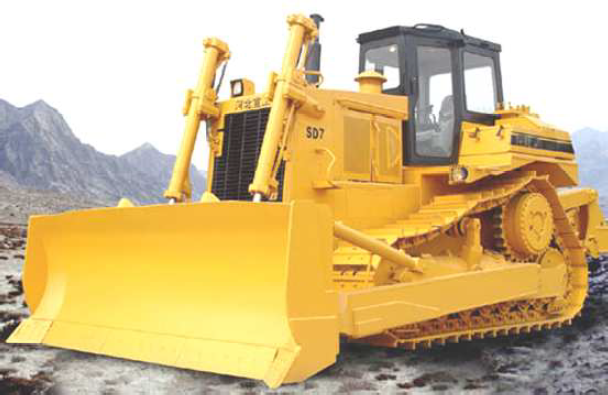
\includegraphics[width=.9\textwidth]{png/img5}
\end{center}
\end{minipage}

\begin{center}
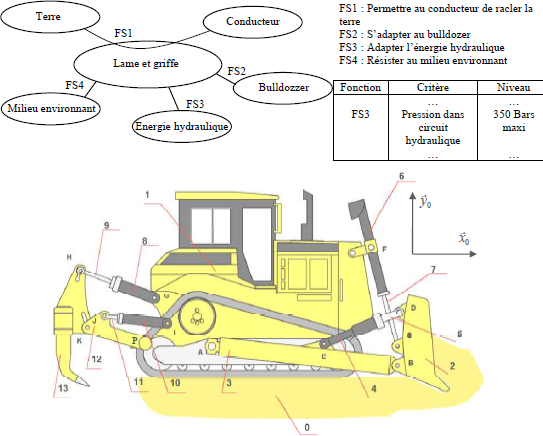
\includegraphics[width=.9\textwidth]{png/img6}
\end{center}

La lame 2 est rattachée au bulldozer 1 par l'intermédiaire de la pièce 3 ainsi que les deux vérins 7+6 et 5+4. La griffe 13 est rattachée au bulldozer par l'intermédiaire de la pièce 12 et du vérin 8+9. Les liaisons aux points $A$, $B$, $C$, $D$, $E$, $F$, $G$, $H$, $I$ et $J$ sont des liaisons pivots parfaites suivant l'axe $\vect{z_0}$. La pièce 12 est reliée à la griffe 13 au point $K$ grâce à une rainure. 

Tous les vérins ont une surface de piston identique de $2\, 500\pi\; mm^2$.

\paragraph{}
\textit{La terre exerce sur la griffe une action mécanique $\vect{F_{\text{sol}\rightarrow \text{griffe}}}$ au point $M$ donnée sur le document réponse. Résoudre graphiquement le problème pour déterminer la pression dans les deux vérins actionnant sur la griffe.}

\textbf{Pour les deux premières questions, vous énoncerez brièvement la démarche utilisée. De plus, vous indiquerez clairement sur le dessin les directions des efforts que vous tracez.}

\paragraph{}
\textit{La terre exerce sur la lame une action mécanique $\vect{F_{\text{sol}\rightarrow \text{lame}}}$ au point $N$ donnée sur le document réponse. Résoudre graphiquement le problème pour déterminer la pression dans les deux vérins actionnant la lame.}


\paragraph{}
\textit{Conclure vis-à-vis du cahier des charges quant aux performances obtenues.}


\newpage 

\begin{center}
\rotatebox{90}{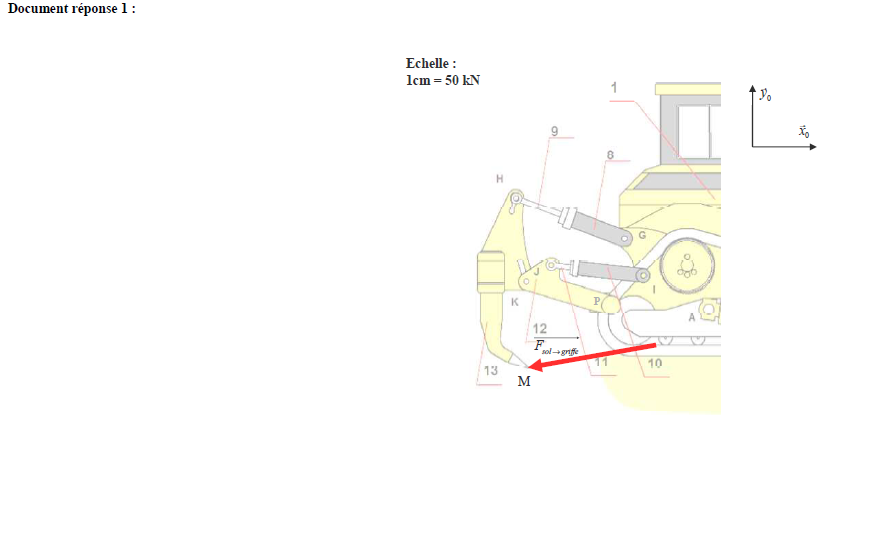
\includegraphics[width=\textheight]{png/img7}}
\end{center}

\newpage 

\begin{center}
\rotatebox{90}{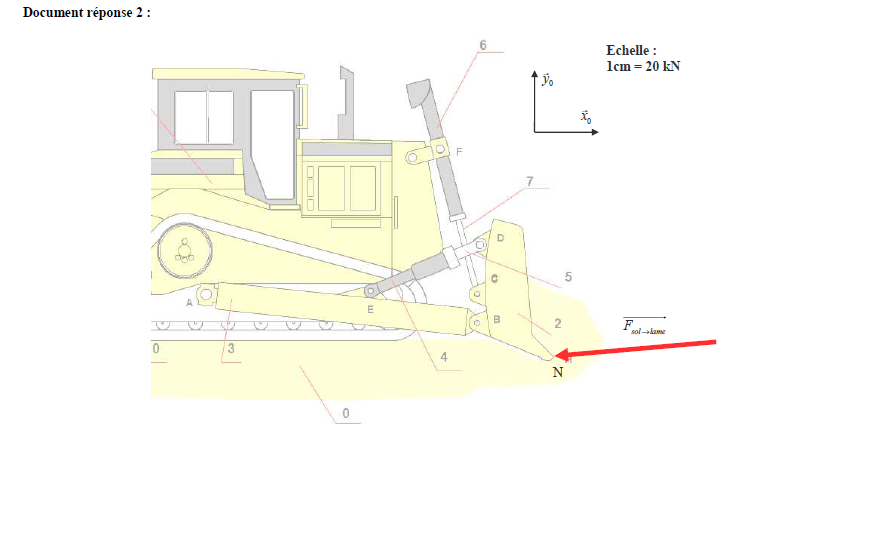
\includegraphics[width=\textheight]{png/img8}}
\end{center}

\newpage

\section*{Echelle en appui sur un mur}
\begin{minipage}[c]{.7\textwidth}
Soit une échelle de longueur $L$ en appui sur un mur. On note $alpha$ l'angle entre l'échelle et le mur. On note $P$ le poids d'une personne montant sur l'échelle. On considère que l'échelle est en contact ponctuel avec le sol et avec le mur.
\end{minipage} \hfill
\begin{minipage}[c]{.25\textwidth}
\begin{center}
\includegraphics[width=\textwidth]{png/echelle}
\end{center}
\end{minipage}

\setcounter{paragraph}{0}
\paragraph{Tous les frottements sont négligés}
\textit{Le grimpeur est situé au milieu de l'échelle. En appliquant le PFS en A à l'ensemble échelle et grimpeur, sans écrire le moindre torseur, montrer que l'échelle ne peut tenir en équilibre.}

\paragraph{On considère qu'il y a du frottement au point $A$.}
\textit{Le coefficient de frottement est égal à 0,3. Reproduire le schéma et faire apparaître le cône de frottement. Préciser la position de l'effort normal et de l'effort tangentiel à la limite du glissement.}
 

\paragraph{On considère qu'il y a du frottement au point $A$.}
\textit{Appliquer le PFS au point A à l'ensemble échelle et grimpeur, déterminer l'angle $\alpha$ pour lequel l'échelle est en équilibre.}

\paragraph{On considère qu'il y a du frottement au point $A$ et en $B$.}
\textit{Dans quelle situation se trouve le système. Pour $\alpha=20^o$, préciser pour quel poids P le système est en équilibre. Vous pourrez utiliser une méthode graphique.}

\end{document}







